%% SR4Rec: SoftwareX Original Software Publication (draft).
%% Build: see paper/README.md. Data figures, tables and numbers come from paper/generated/, which is
%% written by scripts/make_paper_assets.py from finished SR4Rec runs; nothing is typed by hand.
%% Word budget per section is given in comments (main text target: 3,600-3,900 words; limit 4,000).
\documentclass[preprint,12pt]{elsarticle}

\usepackage{lineno}
\usepackage{amssymb,amsmath}
\usepackage{graphicx}
\usepackage{booktabs}
\usepackage{array}
\usepackage{float}
\usepackage{adjustbox}
\usepackage{xcolor}
\usepackage{tikz}
\usetikzlibrary{positioning,arrows.meta,fit,backgrounds}
\usepackage[hidelinks]{hyperref}
\usepackage{url}

\journal{SoftwareX}

% Draft helpers: remove \todo items before submission (grep -n "\\todo" main.tex).
\newcommand{\todo}[1]{\textcolor{red}{[TODO: #1]}}
\newcommand{\pending}[1]{\fbox{\parbox{0.9\linewidth}{\centering\footnotesize\textcolor{red}{Pending: #1}}}}
\newcommand{\generated}[3]{\IfFileExists{generated/#1}{\input{generated/#1}}{\begin{table}[t]\centering\caption{\textcolor{red}{Pending: #2.}}\label{#3}\end{table}}}
\newcommand{\genfig}[3]{\IfFileExists{generated/#1}{\includegraphics[width=#2]{generated/#1}}{\pending{#3}}}
\newcommand{\srfr}{SR4Rec}
\IfFileExists{generated/macros.tex}{% Generated by scripts/make_paper_assets.py. Do not edit.
\newcommand{\DONENumTest}{5,678}
\newcommand{\DONENumClasses}{164}
\newcommand{\DONENumSeeds}{3}
\newcommand{\DONEHours}{13.8}
\newcommand{\DONEDevice}{NVIDIA GeForce RTX 3080}
\newcommand{\DONEFIXEDNumTest}{5,678}
\newcommand{\DONEFIXEDNumClasses}{164}
\newcommand{\DONEFIXEDNumSeeds}{3}
\newcommand{\DONEFIXEDHours}{0.1}
\newcommand{\DONEFIXEDDevice}{NVIDIA GeForce RTX 3080}
\newcommand{\DTWONumTest}{602}
\newcommand{\DTWONumClasses}{62}
\newcommand{\DTWONumSeeds}{3}
\newcommand{\DTWOHours}{0.8}
\newcommand{\DTWODevice}{NVIDIA GeForce RTX 3080}
\newcommand{\DTHREENumTest}{5,794}
\newcommand{\DTHREENumClasses}{200}
\newcommand{\DTHREENumSeeds}{1}
\newcommand{\DTHREEHours}{4.0}
\newcommand{\DTHREEDevice}{NVIDIA GeForce RTX 3080}
\newcommand{\QualCorrected}{793}
\newcommand{\QualDegraded}{993}
}{}
\providecommand{\DONENumTest}{\todo{n}}
\providecommand{\DONENumClasses}{\todo{n}}
\providecommand{\DTWONumClasses}{\todo{n}}
\providecommand{\DONEHours}{\todo{n}}
\providecommand{\DONEDevice}{\todo{n}}
\providecommand{\QualCorrected}{\todo{n}}
\providecommand{\QualDegraded}{\todo{n}}

\begin{document}

\begin{frontmatter}

\title{SR4Rec: A reproducible toolkit for measuring whether super-resolution helps closed-set image recognition}

\author[hcmou]{Thai Le Quang}
\author[hcmou]{V. T. Hoang\corref{cor1}}
\cortext[cor1]{Corresponding author. \todo{e-mail}}
\affiliation[hcmou]{organization={\todo{Faculty, Ho Chi Minh City Open University}},
            city={Ho Chi Minh City},
            country={Vietnam}}

%% 150-200 words. Write last (plan D5.2).
\begin{abstract}
Super-resolution (SR) is often placed in front of recognition models that operate on low-resolution
images, yet SR models are trained and ranked by image-fidelity metrics that do not say whether a
recognizer becomes more accurate. SR4Rec is an open-source Python toolkit that answers this question
for a user's own dataset and SR models. From one configuration file and three commands, it checks
the dataset, builds a closed-set split, produces low-resolution inputs, runs the bicubic baseline and
every SR model, trains a recognizer for each image pipeline, and compares each SR model with bicubic
using paired statistics over test images. The result is a self-contained report with Rank-1, Rank-5,
CMC, macro precision, recall and F1, PSNR and SSIM, results by image size, CPU latency and
before/after-SR panels, together with a fingerprint that makes every number reproducible.
\todo{one or two sentences with the headline findings of D1 and D2, filled from paper/generated/}
Every number in this article is regenerated by one command.
\end{abstract}

\begin{keyword}
super-resolution \sep image recognition \sep biometrics \sep evaluation protocol \sep reproducibility \sep PyTorch
\end{keyword}

\end{frontmatter}

%% ------------------------------------------------------------------------ Required metadata
\section*{Required Metadata}
\label{sec:metadata}

\section*{Current code version}

\begin{table}[H]
\centering
\footnotesize
\begin{tabular}{|l|p{5.4cm}|p{6.2cm}|}
\hline
\textbf{Nr.} & \textbf{Code metadata description} & \textbf{Value} \\
\hline
C1 & Current code version & v0.1.0 \\
\hline
C2 & Permanent link to code/repository used for this code version & \url{https://github.com/OWNER/sr4rec/tree/v0.1.0} \todo{account} \\
\hline
C3 & Permanent link to Reproducible Capsule & \todo{Zenodo DOI of the v0.1.0 archive with checkpoints} \\
\hline
C4 & Legal Code License & MIT \\
\hline
C5 & Code versioning system used & git \\
\hline
C6 & Software code languages, tools, and services used & Python, PyTorch, timm, spandrel, NumPy, SciPy, statsmodels, scikit-learn, pandas, matplotlib, pydantic, Jinja2 \\
\hline
C7 & Compilation requirements, operating environments \& dependencies & Python $\geq$ 3.10; PyTorch $\geq$ 2.3; Linux, Windows or macOS; CUDA or Apple GPU optional; dependencies in \texttt{pyproject.toml} \\
\hline
C8 & If available Link to developer documentation/manual & \url{https://github.com/OWNER/sr4rec\#readme} and \texttt{docs/} \\
\hline
C9 & Support email for questions & \todo{e-mail} \\
\hline
\end{tabular}
\caption{Code metadata (mandatory).}
\label{tab:metadata}
\end{table}

\linenumbers

%% ------------------------------------------------------------------------ 1. Motivation (750-850 words)
\section{Motivation and significance}
\label{sec:motivation}

Recognition from low-resolution images is common in practice: faces and ears captured far from the
camera, animals photographed in the field, or objects cropped from wide-angle scenes. A frequent
remedy is to upscale the input with a super-resolution (SR) model before recognition
\todo{cite 2-3 representative works that use SR as preprocessing for face or ear recognition}.
Modern SR models, from transformer-based restoration networks such as SwinIR~\cite{liang2021swinir}
to models trained for real-world degradations such as Real-ESRGAN~\cite{wang2021realesrgan} and
efficient networks such as SPAN~\cite{wan2024span}, produce visually convincing images. They are,
however, trained and ranked by image-fidelity measures such as PSNR and SSIM~\cite{wang2004ssim} on
natural-image benchmarks. These measures do not tell whether a recognizer becomes more accurate:
an SR model may sharpen edges while altering the fine structures that identify an individual, and
published evidence on the downstream benefit of SR is mixed \todo{cite works reporting gains and works
reporting no gain or harm}.

Answering the question for a given dataset requires a controlled experiment, and such experiments are
easy to get wrong. The recognizer must be trained and evaluated on a closed-set split in which every
identity appears in every split and no image, not even a renamed copy, appears twice. The bicubic
baseline and every SR model must be evaluated on the same test images with the same preprocessing.
Evaluating an existing recognizer on SR outputs measures a domain shift as much as the effect of SR,
so recognizers should also be trained on the images each SR model produces. Differences between SR
models are often small, so they must be tested statistically, over test images and several training
seeds, and reported separately for very small images, where SR matters most. Finally, the outcome
depends on the degradation an SR model was trained for, which is rarely reported next to recognition
results. In our experience each of these steps is re-implemented in ad-hoc scripts for every study,
which makes results hard to compare and to reproduce.

Existing software covers parts of this workflow (Table~\ref{tab:related}). SR toolboxes such as
BasicSR~\cite{basicsr} and KAIR~\cite{kair} train and test SR models and report PSNR and SSIM;
spandrel~\cite{spandrel} loads pretrained SR weights of many architectures; pyiqa~\cite{pyiqa}
computes image-quality metrics; timm~\cite{wightman2019timm} provides recognition backbones; and
opensr-test~\cite{aybar2024opensrtest} benchmarks SR for remote sensing. None of them trains
recognizers under a split and protocol designed for SR, tests the difference with bicubic, or
reports the result by image size. SR4Rec is not a plug-in for an SR toolbox: SR toolboxes train SR
models, whereas SR4Rec treats SR models as fixed inputs and controls the recognition experiment.
Every component could be assembled from these libraries; the contribution of SR4Rec is the
validated workflow that assembles them and the rules it enforces.

\begin{table}[t]
\centering
\footnotesize
\caption{Functionality available after installation. \todo{verify every cell against the current
version of each tool before submission}.}
\label{tab:related}
\setlength{\tabcolsep}{3pt}
\resizebox{\linewidth}{!}{%
\begin{tabular}{lcccccc}
\toprule
 & BasicSR & KAIR & timm & pyiqa & opensr-test & SR4Rec \\
\midrule
Run pretrained SR models & \checkmark & \checkmark & & & \checkmark & \checkmark \\
PSNR / SSIM & \checkmark & \checkmark & & \checkmark & \checkmark & \checkmark \\
Train recognizers & & & \checkmark & & & \checkmark \\
Closed-set split with duplicate checks & & & & & & \checkmark \\
Recognizer trained per SR model (matched protocol) & & & & & & \checkmark \\
Paired statistics against bicubic & & & & & & \checkmark \\
Results by image size & & & & & & \checkmark \\
Native low-resolution images (no HR reference) & & & & \todo{?} & & \checkmark \\
Self-contained report and reproduction command & & & & & \todo{?} & \checkmark \\
\bottomrule
\end{tabular}}
\end{table}

SR4Rec does not propose a new SR method. It provides a measurement instrument with four objectives,
which structure the rest of this article: (O1) a single, validated protocol for the question ``does
this SR model help this recognizer on these data, compared with bicubic?''; (O2) any SR model,
whether a weights file, a PyTorch class or images produced by another tool; (O3) conclusions stated
with statistical support and by image size, including negative results; and (O4) results that anyone
can regenerate with one command. \todo{one sentence on the group's use of the tool, only if the
corresponding paper is accepted or public}

%% ------------------------------------------------------------------------ 2. Software (1100-1200 words)
\section{Software description}
\label{sec:software}

SR4Rec is a Python package built on PyTorch~\cite{paszke2019pytorch}. Users interact with it
through a configuration file, \texttt{sr4rec.yaml}, and three commands: \texttt{sr4rec init} checks a
dataset and writes a fully commented configuration, \texttt{sr4rec run} executes the workflow, and
\texttt{sr4rec reproduce} re-runs a published demonstration and compares the results with the
expected values within stated tolerances.

\subsection{Software architecture}
\label{sec:architecture}

Figure~\ref{fig:architecture} shows the architecture. The command-line interface and the Python API
both construct a single \texttt{Run} object, so they produce identical results. \texttt{Run} calls
six modules in a fixed order. \emph{data} validates the dataset and creates or reads the split;
\emph{lr} produces low-resolution (LR) images; \emph{sr} runs the bicubic baseline and every SR
model; \emph{rec} prepares the recognizer input and trains and evaluates the recognizers;
\emph{eval} and \emph{stats} compute the metrics and the paired tests; and \emph{report} writes the
outputs. The configuration schema is defined once, with pydantic, and the same definition validates
user files, generates the commented file written by \texttt{init}, and generates the configuration
reference in the documentation, so the three cannot diverge. Unknown keys and invalid values are
rejected with the list of accepted values.

Every expensive intermediate result (LR images, SR outputs, splits and trained recognizers) is cached
under a key derived from the content it depends on: SHA-256 hashes of the images and of the SR weights
or code, the configuration of the step, and the split. Re-running a study is therefore fast, adding
an SR model trains only the recognizers of that model, and a stale result cannot be reused by
mistake. Each run also writes \texttt{fingerprint.yaml} with the software and hardware environment
and the hashes of the data and of every weight file.

\begin{figure}[t]
\centering
\resizebox{\linewidth}{!}{% Figure 1: architecture of SR4Rec (TikZ). Included by main.tex.
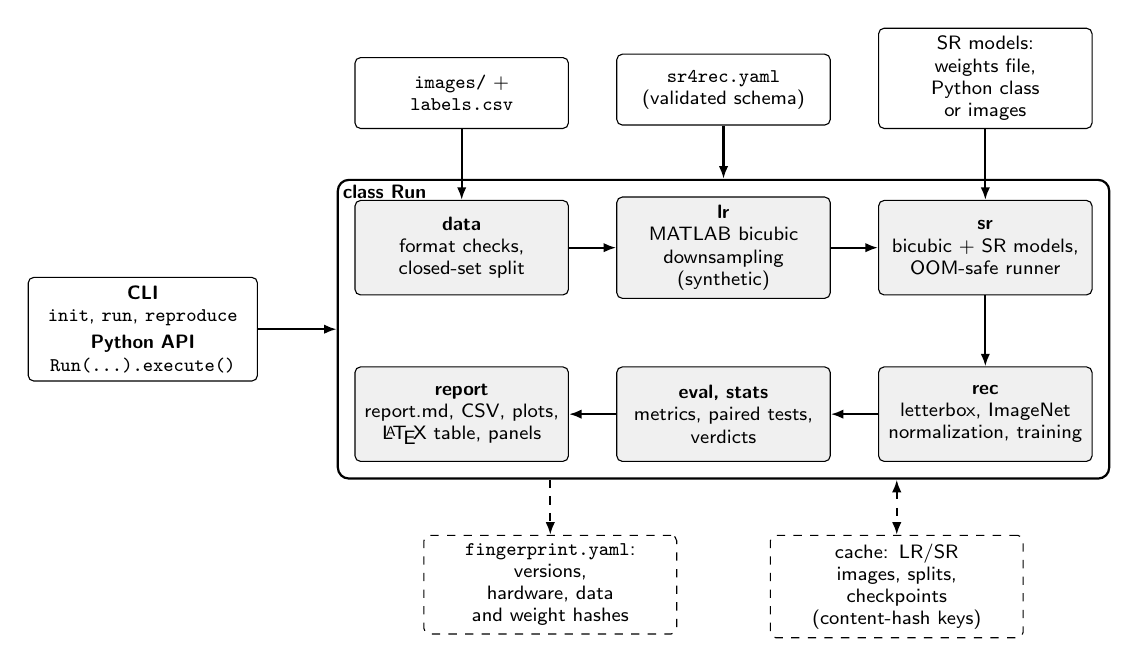
\begin{tikzpicture}[
  font=\sffamily\scriptsize,
  box/.style={draw, rounded corners=2pt, align=center, minimum height=9mm, inner sep=3pt, fill=white},
  mod/.style={box, fill=black!6, text width=25mm, minimum height=12mm},
  io/.style={box, text width=25mm},
  side/.style={box, dashed, text width=30mm},
  arr/.style={-{Latex[length=1.6mm]}, thick},
  node distance=6mm and 6mm]
  % pipeline (two rows)
  \node[mod] (d) {\textbf{data}\\format checks,\\closed-set split};
  \node[mod, right=of d] (lr) {\textbf{lr}\\MATLAB bicubic\\downsampling (synthetic)};
  \node[mod, right=of lr] (sr) {\textbf{sr}\\bicubic + SR models,\\OOM-safe runner};
  \node[mod, below=9mm of sr] (rec) {\textbf{rec}\\letterbox, ImageNet\\normalization, training};
  \node[mod, left=of rec] (ev) {\textbf{eval, stats}\\metrics, paired tests,\\verdicts};
  \node[mod, left=of ev] (rep) {\textbf{report}\\report.md, CSV, plots,\\\LaTeX{} table, panels};
  \begin{scope}[on background layer]
    \node[draw, thick, rounded corners=4pt, fit=(d)(lr)(sr)(rec)(ev)(rep), inner sep=6pt,
          label={[anchor=north west, font=\sffamily\scriptsize\bfseries, inner sep=2pt]north west:class Run}] (run) {};
  \end{scope}
  % inputs above
  \node[io, above=9mm of d] (data) {\texttt{images/} + \texttt{labels.csv}};
  \node[io, above=9mm of lr] (cfg) {\texttt{sr4rec.yaml}\\(validated schema)};
  \node[io, above=9mm of sr] (srin) {SR models: weights file,\\Python class or images};
  % interfaces on the left
  \node[box, left=10mm of run, text width=27mm] (cli) {\textbf{CLI}\\\texttt{init}, \texttt{run}, \texttt{reproduce}\\[2pt]\textbf{Python API}\\\texttt{Run(...).execute()}};
  % side products below
  \node[side, below=7mm of run.south, xshift=-22mm] (fp) {\texttt{fingerprint.yaml}: versions,\\hardware, data and weight hashes};
  \node[side, below=7mm of run.south, xshift=22mm] (cache) {cache: LR/SR images, splits,\\checkpoints (content-hash keys)};
  % arrows
  \draw[arr] (data) -- (d);
  \draw[arr] (cfg) -- (lr.north |- run.north);
  \draw[arr] (srin) -- (sr);
  \draw[arr] (d) -- (lr);
  \draw[arr] (lr) -- (sr);
  \draw[arr] (sr) -- (rec);
  \draw[arr] (rec) -- (ev);
  \draw[arr] (ev) -- (rep);
  \draw[arr] (cli) -- (run);
  \draw[arr, dashed] (fp.north |- run.south) -- (fp.north);
  \draw[arr, dashed, {Latex[length=1.6mm]}-{Latex[length=1.6mm]}] (cache.north |- run.south) -- (cache.north);
\end{tikzpicture}
}
\caption{Architecture of SR4Rec. The CLI and the Python API share one \texttt{Run} class; expensive
steps are cached under content-hash keys; every run writes a report and a fingerprint.}
\label{fig:architecture}
\end{figure}

\subsection{Software functionalities}
\label{sec:functionalities}

\paragraph{Data and split} A dataset is a folder with \texttt{images/} and a \texttt{labels.csv} file
listing the relative path, the label and, optionally, the split of every image. SR4Rec rejects
missing or unreadable files, duplicate paths and classes that are too small, reporting each problem
with its line number. The split comes either from the file or from user-given ratios applied within
every class. Identical images (by SHA-256) are always kept in the same split, and a user-given split
that places identical images in two splits is rejected.

\paragraph{Two data modes} In \emph{synthetic} mode the images are high resolution (HR); SR4Rec
crops them to a multiple of the scale factor and downsamples them with a MATLAB-compatible bicubic
kernel, so PSNR, SSIM and an HR upper bound can be reported. In \emph{native-lr} mode the images
are already small, which is the realistic case for biometrics in the wild, and no downsampling or
fidelity metric is applied.

\paragraph{Three SR sources} An SR model can be given as a weights file whose architecture spandrel
detects, as a Python file with a PyTorch class that follows a four-rule interface
(Section~\ref{sec:snippet}), or as a folder of images produced by any other tool. SR4Rec checks the
scale and the output size of every model before any training (\texttt{run -{}-dry-run}), pads inputs
that are smaller than an architecture requires, and supports tiled inference. The report states the
degradation each validated model was trained for, because a model trained for real-world degradation
is not expected to excel on clean bicubic inputs.

\paragraph{Recognizer input and protocols} Every image, whether bicubic, SR output or HR, is
letterboxed to a square without changing its aspect ratio, padded with the ImageNet mean colour and
normalized with ImageNet statistics~\cite{deng2009imagenet}. Under the default \emph{matched}
protocol, one recognizer is trained per image pipeline, backbone and seed, on the train images of that
pipeline, and selected on its validation images; the test images are never used before evaluation.
The \emph{fixed\_recognizer} protocol trains one recognizer on HR (or bicubic) images and applies
SR at test time only; it is cheaper and answers a different question, which the report states.
Backbones come from timm; ResNet-18~\cite{he2016resnet}, MobileNetV3-Small~\cite{howard2019mobilenetv3}
and ConvNeXt-Tiny~\cite{liu2022convnext} are validated. The training recipe is fixed so that SR
models are compared under identical conditions.

\paragraph{Metrics and statistics} SR4Rec reports Rank-1 accuracy (the primary metric), Rank-5, the
CMC curve, macro precision, recall and F1, and, in synthetic mode, PSNR and SSIM on the Y channel.
For every backbone and SR model, per-image Rank-1 correctness is averaged over seeds and compared
with bicubic on the same images: the difference is given with a 95\% percentile bootstrap
interval~\cite{efron1993bootstrap} and a paired sign-flip permutation test~\cite{good2005permutation},
Holm-corrected~\cite{holm1979} over the SR models of each backbone. A fixed rule turns these into a
verdict: significant gain, significant harm or no difference. The same analysis is repeated in four
bins of LR image size.

\paragraph{Outputs and reproduction} A run folder contains \texttt{report.md}, which answers the
question in at most three rule-generated sentences followed by the tables and figures, the CSV files
behind every number, a \LaTeX{} table, before/after-SR panels for selected test images, and the
fingerprint. \texttt{sr4rec reproduce} runs a published demonstration either in full or, with
\texttt{-{}-eval-only}, from published recognizer checkpoints, and exits with a distinct code when a
metric leaves its tolerance.

\paragraph{Robust execution} SR4Rec uses a CUDA GPU if available, otherwise an Apple GPU, otherwise
the CPU. Running out of GPU memory never stops a run: SR switches to smaller tiles, training to
gradient accumulation with the same effective batch size, evaluation to smaller batches, and, as a
last resort, the step continues on the CPU. Each fallback is listed in the report.

\subsection{Sample code snippet}
\label{sec:snippet}

Listing 1 shows the complete interface for adding an SR model as Python code; the
model is then declared with one line in the configuration
(\texttt{module: sr\_models/tiny\_espcn.py:TinyESPCN}).

{\scriptsize
\begin{verbatim}
class TinyESPCN(torch.nn.Module):
    scale = 4                                   # upscaling factor, checked by SR4Rec

    def __init__(self, weights=None):           # optional weights file
        super().__init__()
        self.body = torch.nn.Sequential(
            torch.nn.Conv2d(3, 32, 5, padding=2), torch.nn.ReLU(),
            torch.nn.Conv2d(32, 3 * self.scale ** 2, 3, padding=1),
            torch.nn.PixelShuffle(self.scale))
        if weights is not None:
            self.load_state_dict(torch.load(weights, weights_only=True))

    def forward(self, x):                       # (N,3,H,W) in [0,1] -> (N,3,4H,4W)
        return self.body(x)
\end{verbatim}}
\noindent{\small Listing 1: an SR model added as a Python class (method 2). SR4Rec verifies the class, the scale and the output shape before use.}\label{lst:module}

\subsection{Technical limitations}
\label{sec:limitations}

Version 0.1 addresses closed-set identification only; verification and open-set protocols, and
attribute classification, are not included. Synthetic degradation is limited to bicubic
downsampling with one scale factor per run. The training recipe is fixed by design, so that all SR models are compared under identical
conditions; per-model tuning is not attempted. CPU latency is not measured for SR models given as images. Runs use one
device.

%% ------------------------------------------------------------------------ 3. Examples (1000-1100 words)
\section{Illustrative examples}
\label{sec:examples}

The numbers in this section are produced by the demonstration configurations shipped with SR4Rec,
frozen with tolerances in the package, and turned into the tables and figures below by
\texttt{scripts/make\_paper\_assets.py}.

\paragraph{Quickstart} SR4Rec installs with \texttt{pip install sr4rec}.
\texttt{sr4rec reproduce quickstart} runs the complete workflow on a small subset of Oxford-IIIT
Pet~\cite{parkhi2012pets} with an SR model given as Python code, on a laptop CPU, in about
\todo{n} minutes. Appendix~B shows the console session for bringing a new dataset through
\texttt{init}, \texttt{run -{}-dry-run} and \texttt{run}; the README walks that path step by step.

\paragraph{Experimental setup} All demonstrations compare bicubic with four validated SR models
at scale 4: SwinIR classical~\cite{liang2021swinir} and SPAN~\cite{wan2024span}, trained for bicubic
degradation, and Real-ESRGAN~\cite{wang2021realesrgan} and SwinIR real-world, trained for real-world
degradation~\cite{zhang2021bsrgan}. The two SwinIR models share one architecture, so their difference
isolates the training degradation. Every run uses the same untuned recipe: an ImageNet-pretrained
ResNet-18~\cite{he2016resnet} fine-tuned for 30 epochs, input 224 $\times$ 224, protocol matched.
D1 uses EarVN1.0~\cite{hoang2019earvn} at its native resolution (\DONENumClasses{} identities,
\DONENumTest{} test images); D2 uses LFW~\cite{huang2007lfw}, people with at least 20 images,
downsampled by 4 (\DTWONumClasses{} identities); D1 and D2 run seeds 0, 1 and 2. D3 is a single run
on CUB-200-2011~\cite{wah2011cub} with its official split and carries no comparative claim. The D1
configuration is listed in full in Appendix~A.

\paragraph{Does SR help on natively small images? (D1)} \todo{2-3 sentences from
Table~\ref{tab:d1}: which SR models changed Rank-1 significantly, with $\Delta$ and CI; say plainly
when the answer is ``no difference''.}

\generated{tab_d1_main.tex}{D1 main results, from scripts/make\_paper\_assets.py}{tab:d1}

\paragraph{Where it helps (D1 by image size)} \todo{2-3 sentences from Figure~\ref{fig:size}: in
which size bins the difference with bicubic changes sign or becomes significant; bins with fewer
than 50 test images are shown but not tested (Appendix~C).}

\begin{figure}[t]
\centering
\genfig{fig_d1_delta_by_size.pdf}{0.8\linewidth}{D1 difference with bicubic by LR size, from scripts/make\_paper\_assets.py}
\caption{D1: Rank-1 difference with bicubic by short side of the LR image, with 95\% bootstrap
intervals over test images; hollow markers are bins with fewer than 50 test images (not tested).}
\label{fig:size}
\end{figure}

\paragraph{What the protocol changes} Running D1 with the \texttt{fixed\_recognizer} protocol, where
one recognizer is trained on bicubic images and SR is applied at test time only, \todo{1-2 sentences:
how the verdicts change relative to Table~\ref{tab:d1} (Table~\ref{tab:summary}); the recognizer then
sees SR outputs outside its training domain while bicubic stays in domain}.

\paragraph{Does image fidelity predict recognition? (D2)} \todo{2-3 sentences from
Table~\ref{tab:d2} and Figure~\ref{fig:fidelity}: whether the ranking by PSNR/SSIM matches the
ranking by Rank-1, and what the SwinIR classical/real-world pair shows about the training
degradation.} No face image is shown in this article.

\generated{tab_d2_fidelity.tex}{D2 fidelity and recognition, from scripts/make\_paper\_assets.py}{tab:d2}

\begin{figure}[t]
\centering
\genfig{fig_d2_fidelity.pdf}{\linewidth}{D2 PSNR/SSIM vs Rank-1, from scripts/make\_paper\_assets.py}
\caption{D2: PSNR and SSIM of each SR model against Rank-1 (mean $\pm$ sd over seeds); marker shape
gives the degradation the model was trained for.}
\label{fig:fidelity}
\end{figure}

\paragraph{Across domains} Table~\ref{tab:summary} collects the demonstrations. \todo{1-2 sentences,
including D3 as a single run.}

\generated{tab_summary.tex}{summary of the demonstrations, from scripts/make\_paper\_assets.py}{tab:summary}

\paragraph{Qualitative results} Figure~\ref{fig:qualitative} shows D1 test images for which an SR
model corrected (rows one and three) or broke (rows two and four) the bicubic prediction, selected
by a fixed rule rather than by hand. Across the test set, \QualCorrected{} images are corrected and
\QualDegraded{} degraded by at least one SR model.

\begin{figure}[t]
\centering
\genfig{fig_d1_qualitative.png}{\linewidth}{D1 before/after-SR panels, from scripts/make\_paper\_assets.py}
\caption{D1: LR input, bicubic, the four SR models; solid green frame: correct identity; dashed
orange frame: wrong identity. Generated by \texttt{scripts/make\_qualitative\_figure.py}, the drawing
function of the \texttt{comparisons/} panels of every report.}
\label{fig:qualitative}
\end{figure}

\paragraph{Deployment} \todo{One sentence on Table~\ref{tab:latency}: the CPU cost of each SR model
relative to the recognizer.} All GPU results come from one \DONEDevice{}.

\generated{tab_latency.tex}{CPU latency, from scripts/make\_paper\_assets.py}{tab:latency}

\paragraph{Reproduction} Reproduction is offered at two levels. \texttt{sr4rec reproduce d1\_earvn
-{}-eval-only}, run against the released recognizer checkpoints, recomputes the SR outputs and the
evaluation \todo{in n minutes and matches the frozen values to n decimal places}. Without the flag
the command retrains the demonstration, \DONEHours{} hours on the reference machine,
\todo{and returns values within the frozen tolerance / identical to the original run}. Both exit with
a distinct code when a metric drifts.

%% ------------------------------------------------------------------------ 4. Impact (400-500 words)
\section{Impact}
\label{sec:impact}

\todo{Whether an SR model is worth putting in front of a recognizer is today settled by trial and
error. SR4Rec makes it a routine measurement; the demonstrations cost \todo{n} GPU-hours. One item
per result of Section~\ref{sec:examples}:}
\begin{itemize}
  \item \todo{whether SR helps on natively small images, and for which sizes (D1);}
  \item \todo{how much the evaluation protocol changes the conclusion (D1, fixed recognizer);}
  \item \todo{whether PSNR/SSIM is a usable proxy for choosing an SR model for recognition (D2).}
\end{itemize}
\todo{Daily practice: what the tool replaces (dataset checks with line numbers, split checks,
dry run, one report), with the effort saved on one task. Use in the group's research only for work
that is accepted or public. Community: frozen expected results, released checkpoints, Zenodo DOI,
semantic versioning, contribution criteria for new validated models, roadmap.}

%% ------------------------------------------------------------------------ 5. Conclusions (150)
\section{Conclusions}
\label{sec:conclusions}

\todo{What SR4Rec does in two sentences; the qualified findings of D1 and D2, negative results
included; every number can be regenerated on demand.}

%% ------------------------------------------------------------------------ Declarations
\section*{CRediT authorship contribution statement}
\textbf{Thai Le Quang:} \todo{Software, Methodology, Investigation, Writing -- original draft}.
\textbf{V. T. Hoang:} \todo{Conceptualization, Supervision, Writing -- review \& editing}.

\section*{Declaration of competing interest}
The authors declare that they have no known competing financial interests or personal relationships
that could have appeared to influence the work reported in this paper.

\section*{Data availability}
The datasets used in the demonstrations are public and must be obtained from their original
sources; SR4Rec provides scripts that convert them. \todo{Zenodo DOI of the archived code, expected
results and recognizer checkpoints.}

\section*{Acknowledgements}
\todo{Funding and acknowledgements.}

%% ------------------------------------------------------------------------ Appendices
\appendix

\section{Configuration of demonstration D1}
\label{app:config}
\todo{\texttt{src/sr4rec/demos/d1\_earvn.yaml} of the release, verbatim.}

\section{Console session}
\label{app:console}
\todo{Transcript of \texttt{sr4rec init}, \texttt{sr4rec run -{}-dry-run}, \texttt{sr4rec run} and
\texttt{sr4rec reproduce} on the quickstart.}

\section{Correctness checks and detailed results}
\label{app:details}
Table~\ref{tab:validation} lists the checks of SR4Rec against reference implementations; the test
suite runs the statistical and metric checks on every change. Table~\ref{tab:d1-size} gives the D1
results per size bin.

\generated{tab_validation.tex}{correctness checks, from paper/validation.yaml}{tab:validation}
\generated{tab_d1_by_size.tex}{D1 results by size bin, from scripts/make\_paper\_assets.py}{tab:d1-size}

\bibliographystyle{elsarticle-num}
\bibliography{references}

\end{document}
